\noindent \textred{3.} 
\begin{figure}[!h]
    \centering
    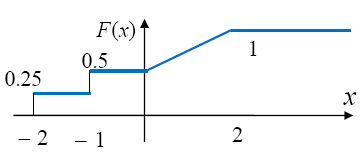
\includegraphics[width=0.5\linewidth]{HWs//HW2//figures/3.png}
\end{figure}
\begin{enumerate}
    \item[(1)] Find and draw $f(x)$. \\
    \myAnswer{
    $f(x) = \underline{0.25[\delta(x+2) + \delta(x+1) + u(x) - u(x-2)]}$ \\
    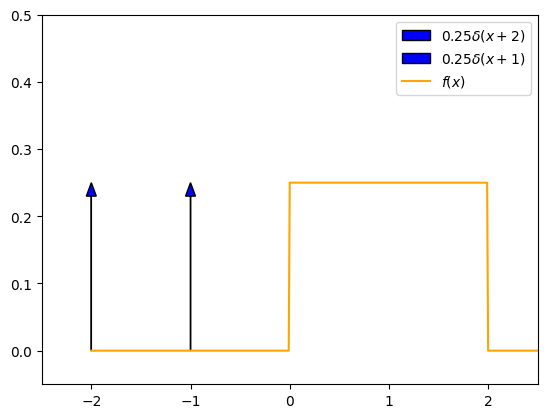
\includegraphics[width=0.5\linewidth]{HWs//HW2//figures/3-1.png}
    }
    \item[(2)] $E\{X\} = \int_{-\infty}^{\infty} x f(x) dx$. Find $E\{X\}$. \\
    \myAnswer{
    \begin{align*}
        E\{X\} &= 0.25 \left\{ \int_{-\infty}^{\infty} x \delta(x+2) dx + \int_{-\infty}^{\infty} x \delta(x+1) dx + \int_{-\infty}^{\infty} x [u(x) - u(x-2)] dx] \right\} \\
        &= 0.25 \times [ (-2) + (-1) + 2 ] = \underline{-0.25}
    \end{align*}
    }
\end{enumerate}